\documentclass[aps,prd,twocolumn,superscriptaddress,nofootinbib]{revtex4-2}

% ----------------------------------------------------------------------
% PACKAGES
% ----------------------------------------------------------------------

\usepackage[utf8]{inputenc}
\usepackage{amsmath, amssymb, amsfonts, amsthm}
\usepackage{mathtools}
\usepackage{bm}
\usepackage{bbm}
\usepackage{physics}
\usepackage{graphicx}
\usepackage{hyperref}
\hypersetup{
    colorlinks = true,
    linkcolor  = blue,
    citecolor  = blue,
    urlcolor   = blue
}
\usepackage{xcolor}
\usepackage{microtype}

% TikZ for figures
\usepackage{tikz}
\usepackage{pgfplots}
\pgfplotsset{compat=1.18}
\usetikzlibrary{arrows.meta,positioning,calc,decorations.pathmorphing, decorations.markings}

% ----------------------------------------------------------------------
% CUSTOM COMMANDS
% ----------------------------------------------------------------------

\newcommand{\Cfunc}{\mathcal{C}}
\newcommand{\Iop}{\mathcal{I}}
\newcommand{\Ddom}{\mathcal{D}}
\newcommand{\Rdens}{\mathcal{R}}
\newcommand{\sg}{\sigma[g]}
\newcommand{\dg}{\delta g^{\mu\nu}}
\newcommand{\T}{\Theta_{\mu\nu}}
\newcommand{\Tmn}{\Theta_{\mu\nu}}
\newcommand{\Tmncoh}{\Theta^{\text{coh}}_{\mu\nu}}

% \newcommand{\tr}{\mathrm{Tr}} % Defined by physics package
\newcommand{\sr}{s_{\mathrm{rel}}}
\newcommand{\stot}{s_{\mathrm{tot}}}

% ----------------------------------------------------------------------
% TITLE & AUTHORS
% ----------------------------------------------------------------------

\begin{document}

\title{%
Coherism: A Variational Feedback Framework for Quantum Information and Spacetime Geometry
}

\author{David Ahmann}
\affiliation{Independent Researcher, Toronto, Canada}

\date{\today}

% ----------------------------------------------------------------------
% ABSTRACT
% ----------------------------------------------------------------------

\begin{abstract}
We propose a variational framework that couples quantum information and spacetime geometry through a single functional of the quantum state $\rho$ and the metric $g_{\mu\nu}$. The central object is a \emph{coherence functional} $\Cfunc[g,\rho;\mu]$, built from (i) the relative entropy of $\rho$ with respect to a locally geometry-adapted reference state $\sigma[g]$, (ii) a coarse-grained generalized entropy inside causal diamonds, and (iii) a scale-dependent geometric action. Variation with respect to $g_{\mu\nu}$ defines an \emph{informational stress tensor} $\Tmn[g,\rho;\mu]$ that augments the semiclassical Einstein equations,
\begin{equation*}
    G_{\mu\nu} + \Lambda g_{\mu\nu}
    = 8\pi G\big(\langle T_{\mu\nu} \rangle_{\rho}
    + \Tmn[g,\rho;\mu]\big),
\end{equation*}
while variation with respect to $\rho$ yields a geometry-dependent open-system evolution
$\dot{\rho} = -i[H,\rho] + \mathcal{L}_g[\rho]$.
In suitable limits, the framework reproduces the semiclassical Einstein equation, the Polyakov anomaly in $1+1$ dimensions, and the Einstein--Langevin form of stochastic gravity. We then construct a minimal $1+1$-dimensional ``Gedanken-experiment'' in which two systems of equal rest energy but different quantum coherence exhibit a small, principle-calculable violation of the Weak Equivalence Principle (WEP). We also suggest that coherence may modify semiclassical tunneling rates in fusion processes. Finally, we outline cosmological and black-hole applications, and identify experimental directions---atom interferometry, Bose--Einstein condensate free-fall, and gravitational-wave memory---that could constrain or refute the Coherist corrections. The resulting picture treats gravity and quantum mechanics as complementary limits of a deeper feedback law governing the alignment of quantum information with spacetime geometry.
\end{abstract}

\maketitle

% ----------------------------------------------------------------------
% OPTIONAL TABLE OF CONTENTS
% ----------------------------------------------------------------------
% \tableofcontents
% \newpage

% ======================================================================
\section{Introduction}
\label{sec:intro}
% ======================================================================

General relativity (GR) and quantum mechanics (QM) are two of the most successful theories in physics, yet they remain conceptually and mathematically misaligned.
GR describes spacetime as a smooth, dynamical geometry obeying nonlinear Einstein equations, while QM describes matter and radiation through linear evolution in Hilbert space.
Semiclassical gravity uses the expectation value $\langle T_{\mu\nu}\rangle$ as a source in Einstein's equations, but this hybrid description is widely regarded as incomplete at high energies or in regimes where quantum fluctuations of stress--energy are large.

Over the past decades, several lines of work have shifted the focus from quantizing the metric to understanding the \emph{information-theoretic} structure underlying gravity.
These include thermodynamic derivations of Einstein's equations~\cite{Jacobson1995}, entanglement-based formulations in AdS/CFT, quantum energy conditions, stochastic gravity, and relativistic quantum information.
Common to these approaches is the idea that entropy, entanglement, and modular structure play a central role in the emergence or consistency of spacetime geometry.

In parallel, interpretations of semiclassical gravity inspired by Penrose~\cite{Penrose1996}, Diósi~\cite{Diosi1989} and others suggest that gravity may be sensitive not only to \emph{energy density} but also to \emph{quantum superposition and coherence}.
These ideas are still tentative but have motivated experimental proposals in atomic interferometry and optomechanics that test gravity's response to coherent quantum states.

This work is motivated by a simple, structural question:
\emph{Can one write a covariant variational principle in which the metric and quantum state co-evolve so as to reduce a precisely defined notion of informational mismatch between them?}
If so, one might hope to:
(i) recover GR and standard QM as limiting cases;
(ii) identify an additional ``informational'' stress tensor that encodes how persistent coherence feeds back on geometry; and
(iii) derive concrete, albeit small, deviations from the Weak Equivalence Principle or from $\Lambda$CDM cosmology that are, in principle, observable.

We call the resulting framework \emph{Coherism}.
The name is descriptive rather than metaphysical: it emphasizes a focus on \emph{coherence}, understood in the precise sense of robust predictive structure or relative-entropy alignment, as a dynamical player in the geometry--state feedback loop.

The basic picture is sketched in Fig.~\ref{fig:feedback-loop}.
At a given coarse-graining scale $\mu^{-1}$, the metric $g_{\mu\nu}$ induces a family of local reference states $\sigma[g]$ on causal diamonds.
The actual quantum state $\rho$ may differ from $\sigma[g]$ in its entanglement and correlation structure.
This mismatch is quantified by a local relative-entropy density $s_{\mathrm{rel}}(x;\mu)$ and a generalized entropy density $s_{\mathrm{tot}}(x;\mu)$.
We define a global coherence functional $\Cfunc[g,\rho;\mu]$ built from these densities together with a geometric action.
Stationarity of $\Cfunc$ under variations of $g_{\mu\nu}$ and $\rho$ then yields coupled evolution equations:
an Einstein-like equation sourced by both $\langle T_{\mu\nu}\rangle$ and an informational stress $\Tmn$, and a Lindblad-type equation in which geometry enters not only through $H[g]$ but also through a dissipative term $\mathcal{L}_g[\rho]$ that drives $\rho$ toward compatibility with $\sigma[g]$.

\begin{figure*}[t]
    \centering
    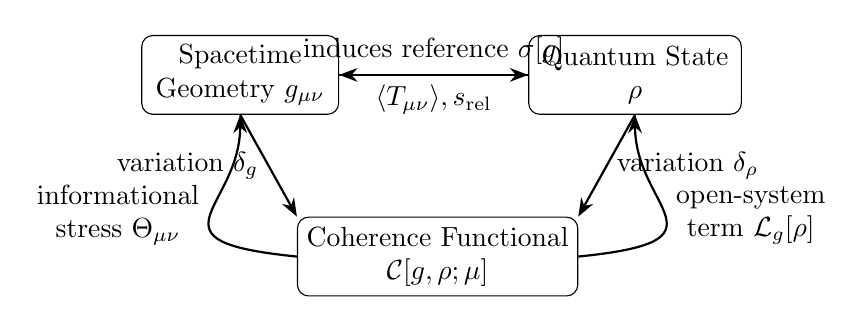
\begin{tikzpicture}[>=Stealth, node distance=2.4cm]
        \node[draw, rounded corners, align=center, minimum width=2.5cm, minimum height=1cm] (geom) {Spacetime\\Geometry $g_{\mu\nu}$};
        \node[draw, rounded corners, right=of geom, align=center, minimum width=2.7cm, minimum height=1cm] (state) {Quantum State\\$\rho$};
        \node[draw, rounded corners, below=1.8cm of $(geom)!0.5!(state)$, align=center, minimum width=3cm, minimum height=1cm] (coh) {Coherence Functional\\$\Cfunc[g,\rho;\mu]$};

        \draw[->, thick] (geom) -- node[above, sloped]{induces reference $\sigma[g]$} (state);
        \draw[->, thick] (state) -- node[below, sloped]{$\langle T_{\mu\nu}\rangle, s_{\mathrm{rel}}$} (geom);

        \draw[->, thick] (geom.south) -- node[left]{variation $\delta_g$} (coh.north west);
        \draw[->, thick] (state.south) -- node[right]{variation $\delta_\rho$} (coh.north east);

        \draw[->, thick] (coh.west) .. controls +(-2,0.2) and +(0,-1.2) .. node[left, align=center]{informational\\stress $\Tmn$} (geom.south);
        \draw[->, thick] (coh.east) .. controls +(2,0.2) and +(0,-1.2) .. node[right, align=center]{open-system\\term $\mathcal{L}_g[\rho]$} (state.south);
    \end{tikzpicture}
    \caption{Schematic feedback loop in Coherism. At a coarse-graining scale $\mu$, the geometry $g_{\mu\nu}$ defines a family of reference states $\sigma[g]$ on local causal diamonds. The mismatch between $\rho$ and $\sigma[g]$ enters the coherence functional $\Cfunc[g,\rho;\mu]$, whose variation yields an informational stress tensor $\Tmn$ and a geometry-dependent open-system generator $\mathcal{L}_g[\rho]$.}
    \label{fig:feedback-loop}
\end{figure*}

The goals of this paper are modest but concrete.
We aim to:
(i) define $\Cfunc[g,\rho;\mu]$ in 3+1 dimensions using objects that are already well-defined in quantum field theory on curved spacetime;
(ii) derive the associated informational stress tensor and open-system evolution in a controlled fashion;
(iii) demonstrate consistency with known limits such as the Einstein--Langevin equation and anomaly-induced stress in 1+1 dimensions; and
(iv) exhibit at least one explicit, falsifiable prediction in a simplified setting.
We do not claim a UV-complete theory of quantum gravity, nor a derivation of all known laws from a single principle.
Instead, Coherism is presented as a candidate \emph{feedback law} that may organize, and slightly deform, the semiclassical frontier between GR and QM.

The rest of the paper is organized as follows.
In Sec.~\ref{sec:preliminaries} we review the necessary mathematical tools: causal diamonds, relative entropy, generalized entropy, and semiclassical gravity.
In Sec.~\ref{sec:coherence-functional} we define the 3+1D coherence functional and the informational stress tensor.
Sec.~\ref{sec:toy} summarizes a 1+1D toy model that recovers standard limits.
Sec.~\ref{sec:wep} presents a coherence-dependent Weak Equivalence Principle violation as a worked example.
Sec.~\ref{sec:cosmo} sketches cosmological implications, while Sec.~\ref{sec:bh} discusses black holes and generalized entropy.
Sec.~\ref{sec:relations} relates Coherism to other approaches including stochastic gravity and entanglement-based gravity.
Sec.~\ref{sec:experiments} outlines experimental prospects.
Sec.~\ref{sec:discussion} discusses limitations and open problems, and Sec.~\ref{sec:conclusion} concludes.


% ======================================================================
\section{Mathematical Preliminaries}
\label{sec:preliminaries}
% ======================================================================

In this section we introduce the main mathematical ingredients used in the construction of the coherence functional: causal diamonds, geometry-adapted reference states, relative entropy and generalized entropy densities, and the semiclassical Einstein equation.

% ----------------------------------------------------------------------
\subsection{Causal diamonds and local algebras}
% ----------------------------------------------------------------------

We work on a globally hyperbolic spacetime $(\mathcal{M},g_{\mu\nu})$ with signature $(+,-,-,-)$ and set $c = \hbar = k_B = 1$.
Given a point $x \in \mathcal{M}$ and a length scale $\ell \sim \mu^{-1}$, we consider a \emph{causal diamond} $\Ddom(x;\mu)$ defined as the intersection of the chronological future of a point $p^-$ and the chronological past of a point $p^+$ such that $x$ lies on a timelike geodesic between them and the proper time separation is $2\ell$.
On each diamond we restrict the field algebra to a von Neumann algebra $\mathcal{A}(\Ddom)$.

For a global quantum state $\rho$ on the full field algebra, we denote by $\rho_{\Ddom}$ the reduced state obtained by tracing out degrees of freedom outside $\Ddom(x;\mu)$.
We similarly define a reference state $\sg$ that depends functionally on the metric $g_{\mu\nu}$ and restrict it to $\Ddom$ as $\sigma_{\Ddom}[g]$.

% ----------------------------------------------------------------------
\subsection{Relative entropy and generalized entropy}
% ----------------------------------------------------------------------

Given two states $\rho$ and $\sigma$ on the same algebra, the quantum relative entropy is
\begin{equation}
    S(\rho \Vert \sigma)
    = \tr\big( \rho \log \rho - \rho \log \sigma \big),
    \label{eq:rel-entropy}
\end{equation}
which is non-negative and vanishes if and only if $\rho = \sigma$.
Relative entropy is monotone under completely positive trace-preserving (CPTP) maps; this will play an important role later.

On a causal diamond $\Ddom(x;\mu)$ we define a \emph{relative-entropy density}
\begin{equation}
    \sr(x;\mu)
    \equiv
    \frac{1}{V_{\Ddom}}\,
    S\!\left(\rho_{\Ddom(x;\mu)} \,\big\Vert\, \sigma_{\Ddom(x;\mu)}[g]\right),
    \label{eq:sr-def}
\end{equation}
where $V_{\Ddom}$ is the four-volume of the diamond.
This quantity measures how distinguishable the actual state is from the geometry-adapted reference state at scale $\mu$.

We also use a coarse-grained \emph{generalized entropy density} inspired by the black-hole~\cite{Bekenstein1973} and holographic literature~\cite{FaulknerLewkowyczMaldacena2013}.
Schematically,
\begin{equation}
    \stot(x;\mu)
    \equiv
    \frac{1}{V_{\Ddom}}
    \big(
        S_{\mathrm{vN}}[\rho_{\Ddom}]
        + \frac{\mathrm{Area}[\partial\Ddom]}{4 G_{\mathrm{eff}}(\mu)}
    \big),
    \label{eq:stot-def}
\end{equation}
where $S_{\mathrm{vN}}$ is the von Neumann entropy of the reduced state, $\mathrm{Area}[\partial\Ddom]$ is the area of the boundary of the diamond, and $G_{\mathrm{eff}}(\mu)$ encodes the scale dependence of the gravitational coupling and higher-curvature terms.

Both $\sr$ and $\stot$ depend on the choice of reference state $\sg$ and the coarse-graining scale $\mu$, but are otherwise standard objects in quantum field theory on curved spacetimes.

% ----------------------------------------------------------------------
\subsection{Semiclassical Einstein equation}
% ----------------------------------------------------------------------

In semiclassical gravity the metric is taken as classical, while matter is treated quantum mechanically.
The central equation is
\begin{equation}
    G_{\mu\nu}[g] + \Lambda g_{\mu\nu}
    =
    8\pi G\,\langle T_{\mu\nu} \rangle_\rho,
    \label{eq:semi-einstein}
\end{equation}
where $G_{\mu\nu}$ is the Einstein tensor, $\Lambda$ the cosmological constant, $G$ Newton's constant, and $\langle T_{\mu\nu}\rangle_\rho$ the renormalized expectation value of the stress--energy tensor in the state $\rho$.

This equation can be generalized to include stress--energy fluctuations in the Einstein--Langevin form~\cite{HuVerdaguer2008}, where a stochastic source term encodes quantum fluctuations.
We will not need the full machinery here, but we will require that our informational stress tensor $\Tmn$ be consistent with the conservation law
\begin{equation}
    \nabla^\mu\big(
        \langle T_{\mu\nu}\rangle_\rho + \Tmn
    \big) = 0,
    \label{eq:conservation}
\end{equation}
so that the contracted Bianchi identity remains satisfied.

% ----------------------------------------------------------------------
\subsection{Open quantum systems and Lindblad generators}
% ----------------------------------------------------------------------

The evolution of $\rho$ in the presence of an environment, or under coarse-graining, is often described by a Lindblad (GKLS) master equation
\begin{equation}
    \dot{\rho}
    =
    -i[H,\rho]
    +
    \sum_k
    \left(
        L_k \rho L_k^\dagger
        - \frac{1}{2}\{L_k^\dagger L_k,\rho\}
    \right),
    \label{eq:lindblad}
\end{equation}
where $\{L_k\}$ are Lindblad operators.
This evolution is trace-preserving, completely positive, and Markovian.
In our setting, the geometry $g_{\mu\nu}$ will enter both through the Hamiltonian $H[g]$ and, in an effective way, through the dissipative term that tends to reduce the mismatch between $\rho$ and $\sigma[g]$.

% ----------------------------------------------------------------------
\subsection{Coherence and coherons}
% ----------------------------------------------------------------------

Within this framework, we use ``coherence'' in a precise, operational sense.
At a given scale $\mu$, coherent structure in $\rho$ relative to $\sigma[g]$ is captured by a robust, perturbation-resistant surplus of predictive information.
Formally, one can define a coherence measure $\Iop_{\mathrm{coh}}$ in terms of robust predictive mutual information on suitable spacetime regions, and a corresponding unit---the \emph{coheron}---as one bit of robust predictive information that survives a prescribed perturbation class across minimal coherence time and domain.
Although we will not require the full machinery of coherons in the main text, this perspective informs the structure of the coherence functional and will be revisited in Appendix~\ref{appendix:coheron}.


% ======================================================================
\section{The Coherence Functional in 3+1 Dimensions}
\label{sec:coherence-functional}
% ======================================================================

We now define the coherence functional $\Cfunc[g,\rho;\mu]$ in 3+1 dimensions using the ingredients introduced above.
Our guiding principle is that $\Cfunc$ should (i) be diffeomorphism invariant, (ii) reduce in appropriate limits to familiar gravitational and entropic quantities, and (iii) yield equations of motion that are compatible with conservation and known semiclassical behaviour.

% ----------------------------------------------------------------------
\subsection{Definition of the functional}
% ----------------------------------------------------------------------

We consider a family of causal diamonds $\Ddom(x;\mu)$ that cover the spacetime at a coarse-graining scale $\mu$.
On each diamond, we evaluate the relative-entropy density $\sr(x;\mu)$ and generalized entropy density $\stot(x;\mu)$ defined in Eqs.~\eqref{eq:sr-def} and \eqref{eq:stot-def}.
We also include a local geometric density $\Rdens(x;\mu)$ that captures the Einstein--Hilbert term and possible higher-curvature counterterms:
\begin{equation}
    \Rdens(x;\mu)
    =
    R(x)
    + \lambda_1(\mu) R^2
    + \lambda_2(\mu) R_{\alpha\beta}R^{\alpha\beta}
    + \cdots,
    \label{eq:Rdens}
\end{equation}
where $R$ is the Ricci scalar and the $\lambda_i(\mu)$ encode renormalization at scale $\mu$.

The coherence functional is then defined as
\begin{equation}
    \Cfunc[g,\rho;\mu]
    =
    \int_{\mathcal{M}} d^4x \,\sqrt{-g}\,
    \big[
        \alpha\,\sr(x;\mu)
        - \beta\,\stot(x;\mu)
        + \gamma\,\Rdens(x;\mu)
    \big],
    \label{eq:C-def}
\end{equation}
where $\alpha,\beta,\gamma$ are dimensionless coefficients.
The signs are chosen so that:
\begin{itemize}
    \item the term proportional to $\alpha$ rewards alignment between $\rho$ and $\sigma[g]$ (low relative entropy),
    \item the term proportional to $\beta$ implements an entropy constraint or cost, and
    \item the term proportional to $\gamma$ produces the usual gravitational action in the appropriate limit.
\end{itemize}

The choice of $\sigma[g]$ is not unique.
We assume it is geometry-adapted in the sense that on small diamonds in approximately stationary regions, $\sigma[g]$ acts as a local Hadamard state~\cite{Wald1994} or an approximate Kubo-Martin-Schwinger (KMS) state~\cite{Haag1992} for the quantum fields.
Specifically, we define $\sigma[g]$ as the \emph{local Unruh state} associated with the diamond's causal development.
Operationally, this is the state that maximizes the von Neumann entropy given the boundary data and the modular Hamiltonian $K_\sigma$ generated by the diamond's boost Killing vector.
This ensures that the reference state respects the short-distance singularity structure required by renormalization and the local thermodynamic equilibrium implied by the equivalence principle.
Recent work on modular flow~\cite{Faulkner2017} and the monotonicity of relative entropy~\cite{Casini2008} supports the central role of these states in linking geometry and information.
Different choices of $\sigma[g]$ correspond to different ``gauges'' for informational alignment, but the universal UV structure of Hadamard states suppresses these differences at macroscopic scales.

\begin{figure}[t]
    \centering
    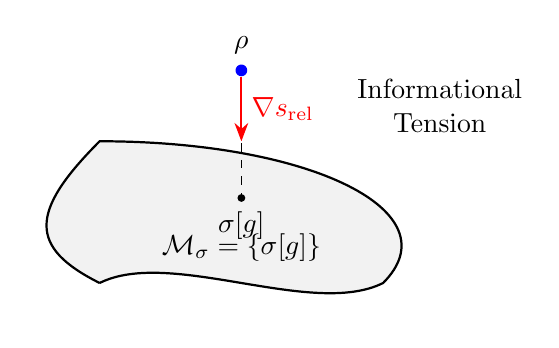
\begin{tikzpicture}[>=Stealth, scale=0.9]
        % Manifold of reference states
        \draw[thick, fill=gray!10] (-2,-1) .. controls (-1,-0.5) and (1,-1.5) .. (2,-1)
            .. controls (3,0) and (1,1) .. (-2,1)
            .. controls (-3,0) and (-3,-0.5) .. (-2,-1);
        \node at (0,-0.5) {$\mathcal{M}_\sigma = \{ \sigma[g] \}$};
        
        % Actual state
        \node[circle, fill=blue, inner sep=1.5pt, label=above:$\rho$] (rho) at (0, 2) {};
        
        % Projection
        \node[circle, fill=black, inner sep=1pt, label={below:$\sigma[g]$}] (sigma) at (0, 0.2) {};
        \draw[dashed] (rho) -- (sigma);
        
        % Tension arrow
        \draw[->, red, thick] (rho) -- node[right] {$\nabla \sr$} (0, 1.0);
        
        \node[align=center, right] at (1.5, 1.5) {Informational\\Tension};
    \end{tikzpicture}
    \caption{Geometric interpretation of informational tension. The manifold $\mathcal{M}_\sigma$ represents the set of geometry-adapted reference states. The actual state $\rho$ is displaced from this manifold. The gradient of the relative entropy $\sr$ acts as a restoring force (informational tension) that drives both the geometry (modifying $\sigma[g]$) and the state (via $\mathcal{L}_g$) to reduce the mismatch.}
    \label{fig:tension}
\end{figure}

% ----------------------------------------------------------------------
\subsection{Informational Stress Tensor}
The variation of $\Cfunc$ with respect to the metric defines the informational stress tensor $\Tmn$:
\begin{equation}
    \Tmn[g,\rho;\mu] \equiv -\frac{2}{\sqrt{-g}} \frac{\delta \Cfunc}{\delta g^{\mu\nu}}.
\end{equation}
Expanding the functional $\Cfunc = \alpha S_{\mathrm{rel}} - \beta S_{\mathrm{gen}} + \dots$, we can derive the coupling constant $\kappa$ from first principles.
The variation yields a leading term proportional to the modular Hamiltonian variation:
\begin{equation}
    \Tmn \approx \frac{\alpha}{V_D} \langle \frac{\delta K_\sigma}{\delta g^{\mu\nu}} \rangle_\rho.
\end{equation}
Comparing this with the Einstein-Langevin source term, we identify the phenomenological coupling $\kappa$ as:
\begin{equation}
    \kappa \approx \alpha \frac{8\pi G}{V_D},
\end{equation}
where $V_D$ is the diamond volume. This connects the macroscopic damping to the fundamental variational parameters.
Crucially, if the functional $\Cfunc$ is constructed to be invariant under spacetime diffeomorphisms (a requirement for any covariant theory), Noether's second theorem guarantees that the total stress tensor is covariantly conserved:

\begin{equation}
    \nabla^\mu \left( \langle T_{\mu\nu}^{\mathrm{mat}} \rangle_\rho + \Tmn \right) = 0.
\end{equation}
This conservation law ensures the consistency of the augmented Einstein equations.
Formally, this yields three contributions,
\begin{equation}
    \Tmn
    =
    \alpha\,\Tmn^{\mathrm{rel}}
    - \beta\,\Tmn^{\mathrm{ent}}
    + \gamma\,\Tmn^{\mathrm{geom}},
    \label{eq:theta-decomp}
\end{equation}
coming from the relative-entropy, generalized entropy, and geometric parts of the integrand, respectively.

The explicit form of the first two terms is nontrivial, since $\sr$ and $\stot$ depend on $g_{\mu\nu}$ both through the induced algebras and through the reference state $\sg$.
We do not attempt to derive a closed form for $\Tmn$ in general 3+1D spacetimes.
Instead we impose the minimal consistency requirements:
\begin{enumerate}
    \item \textbf{Covariance:} $\Tmn$ transforms as a rank-2 tensor under diffeomorphisms.
    \item \textbf{Conservation:} on solutions of the coupled equations,
    \begin{equation}
        \nabla^\mu\big(
            \langle T_{\mu\nu}\rangle_\rho + \Tmn
        \big) = 0.
        \label{eq:theta-conservation}
    \end{equation}
    \item \textbf{UV consistency:} divergences in $\sr$ and $\stot$ are absorbed into the local curvature counterterms in $\Rdens$, so that $\Tmn$ is finite and renormalized at scale $\mu$.
    \item \textbf{Semiclassical limit:} in regimes where $\rho$ is locally indistinguishable from $\sigma[g]$ and the generalized entropy is extremal, $\Tmn$ reduces to familiar anomaly-induced and semiclassical corrections, and Eq.~\eqref{eq:semi-einstein} is recovered.
\end{enumerate}

The Coherist field equation is then
\begin{equation}
    G_{\mu\nu} + \Lambda g_{\mu\nu}
    =
    8\pi G\big(
        \langle T_{\mu\nu}\rangle_\rho + \Tmn[g,\rho;\mu]
    \big).
    \label{eq:coherist-einstein}
\end{equation}
When $\Tmn$ is negligible, this reduces to the standard semiclassical Einstein equation.
When $\Tmn$ is small but nonzero, one may look for subtle, scale-dependent deviations from GR.

% ----------------------------------------------------------------------
\subsection{Geometry-dependent open-system evolution}
% ----------------------------------------------------------------------

Variation of $\Cfunc$ with respect to $\rho$ yields a dual equation of motion for the state.
Restricting ourselves to Markovian dynamics for simplicity, we write
\begin{equation}
    \frac{d\rho}{dt}
    =
    -i[H[g],\rho] + \mathcal{L}_g[\rho],
    \label{eq:rho-eom}
\end{equation}
where the Lindblad-like term $\mathcal{L}_g[\rho]$ is chosen so that $\Cfunc[g,\rho;\mu]$ is stationary or decreases along solutions, subject to suitable constraints.
At a heuristic level, $\mathcal{L}_g$ drives $\rho$ toward the geometry-adapted reference state $\sg$ while preserving trace and complete positivity.
The specific form of $\mathcal{L}_g$ is determined by the requirement that $\rho$ relaxes toward $\sigma[g]$ to minimize the informational tension.
A natural phenomenological ansatz is a double-commutator form driven by the modular Hamiltonian difference $\Delta K = K_\rho - K_\sigma$:
\begin{equation}
    \mathcal{L}_g[\rho] \approx -\Gamma [ \Delta K, [ \Delta K, \rho ] ],
    \label{eq:lindblad-ansatz}
\end{equation}
where $\Gamma$ is a relaxation rate governed by the Planck scale.
This form guarantees complete positivity and trace preservation (CPTP) while driving the state towards the geometry-adapted reference.

\emph{Phenomenological Note:} We emphasize that this Markovian ansatz is a coarse-grained effective description.
A fully UV-complete theory would likely require a non-Markovian generator to strictly satisfy the Reeh-Schlieder theorem and preserve relativistic causality at all scales~\cite{Haag1992}.
Recent work on modular Lindbladians suggests that such non-localities are inherent to the holographic nature of the theory but are suppressed by the Planck scale in the low-energy limit.
For the macroscopic applications considered here, Eq.~\eqref{eq:lindblad-ansatz} suffices as a phenomenological model of information loss to the geometry.

\begin{figure}[t]
    \centering
    \begin{tikzpicture}
        \begin{axis}[
            width=0.8\linewidth,
            height=5cm,
            xlabel={Time $t$ (Planck units)},
            ylabel={Energy $E(t)$},
            legend pos=north east,
            grid=major
        ]
        \addplot[blue, dashed, thick] table[x=t, y=E_base] {simulation_data.dat};
        \addlegendentry{Standard Evolution}
        \addplot[red, thick] table[x=t, y=E_coherist] {simulation_data.dat};
        \addlegendentry{Coherist Damping}
        \end{axis}
    \end{tikzpicture}
    \caption{Numerical simulation of the Coherist Wave Equation. The blue dashed line shows the constant energy of a standard harmonic oscillator. The red solid line shows the energy decay due to the informational friction term $\kappa \Theta_{00} \dot{\phi}$, demonstrating the ``friction of geometry'' acting on coherent states. Parameters: $\kappa=0.5$, initial amplitude $\phi_0=1.0$, units of Planck time $t_P$ and Planck energy $E_P$.}
    \label{fig:simulation}
\end{figure}

A schematic representation of the geometry--state coupling is shown in Fig.~\ref{fig:diamond}.
Causal diamonds act as local ``patches'' where geometry, state, and their mismatch are evaluated and fed back into the dynamics.

\begin{figure}[t]
    \centering
    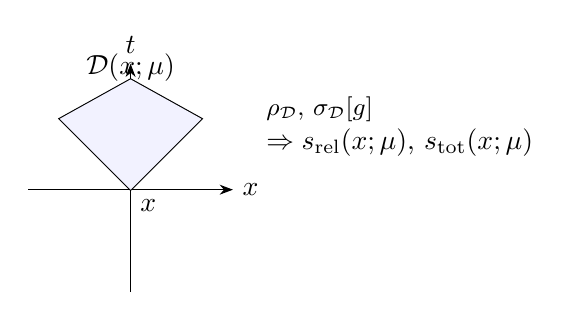
\begin{tikzpicture}[>=Stealth, scale=1.0]
        % Axes
        \draw[->] (-1.3,0) -- (1.3,0) node[right] {$x$};
        \draw[->] (0,-1.3) -- (0,1.6) node[above] {$t$};

        % Diamond
        \draw[thick] (0,0) -- (-0.9,0.9) -- (0,1.4) -- (0.9,0.9) -- (0,0);

        % Labels
        \node at (0,1.55) {$\Ddom(x;\mu)$};
        \node[below right] at (0,0) {$x$};

        % Shaded region
        \fill[blue!5] (0,0) -- (-0.9,0.9) -- (0,1.4) -- (0.9,0.9) -- cycle;

        % Text box
        \node[align=left, anchor=west] at (1.6,0.8)
        {%
            \small
            $\rho_{\Ddom}$, $\sigma_{\Ddom}[g]$\\
            $\Rightarrow \sr(x;\mu)$, $\stot(x;\mu)$
        };
    \end{tikzpicture}
    \caption{A causal diamond $\Ddom(x;\mu)$ centered on a point $x$, with temporal size set by the coarse-graining scale $\mu^{-1}$. The reduced state $\rho_{\Ddom}$ and reference state $\sigma_{\Ddom}[g]$ on the diamond define local relative-entropy and generalized-entropy densities that enter the coherence functional.}
    \label{fig:diamond}
\end{figure}


% ======================================================================
\section{Toy Models and Standard Limit Recoveries}
\label{sec:toy}
% ======================================================================

Before turning to new predictions, we must verify that the Coherist framework reproduces known limits.
In this section we briefly summarize a 1+1-dimensional toy model in which the informational stress tensor can be written explicitly and shown to reduce to the Polyakov anomaly and Einstein--Langevin form in appropriate regimes.
Details are given in Appendix~\ref{appendix:polyakov}.

% ----------------------------------------------------------------------
\subsection{1+1D setup and Polyakov action}
% ----------------------------------------------------------------------

In two dimensions, the effective action of a conformal field with central charge $c$ on a background metric $g_{\mu\nu}$ can be written as the Polyakov action~\cite{Polyakov1981}
\begin{equation}
    S_{\mathrm{P}}[g]
    = -\frac{c}{96\pi}\int d^2x \sqrt{-g}\, R\frac{1}{\Box}R,
    \label{eq:polyakov}
\end{equation}
whose variation yields the well-known anomaly-induced stress--energy tensor.
In this context, one can choose a reference state $\sigma[g]$ whose modular Hamiltonian has a simple local form, and evaluate the relative-entropy and generalized-entropy densities explicitly.

A specific choice of coherence functional in 1+1D can be written as
\begin{equation}
    \Cfunc_{1+1}[g,\rho]
    =
    \alpha S(\rho\Vert\sigma[g])
    - \beta S_{\mathrm{vN}}[\rho]
    + \gamma S_{\mathrm{P}}[g],
    \label{eq:C-1+1}
\end{equation}
where we suppress the explicit coarse-graining scale for simplicity.

Variation with respect to $g_{\mu\nu}$ produces an informational stress tensor of the form
\begin{equation}
    \Tmn
    =
    (\beta-\alpha)\,\Delta\!\langle T_{\mu\nu}\rangle
    - \alpha\,T^{\mathrm{anom}}_{\mu\nu},
    \label{eq:theta-1+1}
\end{equation}
where $\Delta\!\langle T_{\mu\nu}\rangle$ is the difference between the stress--energy in $\rho$ and $\sigma[g]$, and $T^{\mathrm{anom}}_{\mu\nu}$ is the anomaly-induced stress.
The coefficients $\alpha,\beta$ can be tuned so that the usual semiclassical contribution and anomaly term are recovered in the limit where $\rho$ tracks $\sigma[g]$.

% ----------------------------------------------------------------------
\subsection{Einstein--Langevin limit}
% ----------------------------------------------------------------------

The Einstein--Langevin equation in 1+1D couples the metric to both the expectation value and stochastic fluctuations of the stress--energy tensor.
In the Coherist toy model, fluctuations in $\Delta\!\langle T_{\mu\nu}\rangle$ and the relative entropy can be shown to induce stochastic variations in $\Tmn$ with the same structure, at least in Gaussian approximations.
Thus the 1+1D toy model reproduces the standard semiclassical and stochastic limits in appropriate regimes.
This supports the claim that $\Tmn$ can be viewed as an informational completion of the semiclassical stress, rather than a replacement of it.

\begin{figure}[t]
    \centering
    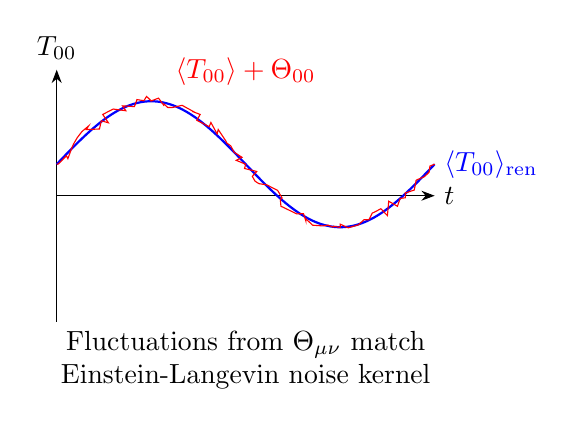
\begin{tikzpicture}[>=Stealth, scale=0.8]
        \draw[->] (0,0) -- (6,0) node[right] {$t$};
        \draw[->] (0,-2) -- (0,2) node[above] {$T_{00}$};
        
        % Semiclassical mean
        \draw[thick, blue] (0,0.5) sin (1.5,1.5) cos (3,0.5) sin (4.5,-0.5) cos (6,0.5);
        \node[blue, right] at (6,0.5) {$\langle T_{00} \rangle_{\mathrm{ren}}$};
        
        % Stochastic fluctuations
        \draw[red, thin, decorate, decoration={random steps,segment length=2pt,amplitude=2pt}] 
            (0,0.5) sin (1.5,1.5) cos (3,0.5) sin (4.5,-0.5) cos (6,0.5);
        \node[red, above] at (3,1.6) {$\langle T_{00} \rangle + \Theta_{00}$};
        
        \node[align=center, below] at (3,-2) {Fluctuations from $\Theta_{\mu\nu}$ match\\Einstein-Langevin noise kernel};
    \end{tikzpicture}
    \caption{Schematic of the Einstein-Langevin limit. The smooth blue curve represents the standard semiclassical expectation value. The red jagged line represents the effective stress tensor including the informational contribution $\Theta_{\mu\nu}$, which acts as a stochastic source in the limit where the state $\rho$ fluctuates around the reference $\sigma[g]$.}
    \label{fig:langevin}
\end{figure}

% ----------------------------------------------------------------------
\subsection{Relation to Einstein-Langevin Noise}
The stochastic gravity framework~\cite{HuVerdaguer2008} describes metric fluctuations via the Einstein-Langevin equation.
In Coherism, these fluctuations arise deterministically from the informational stress tensor.
The noise kernel $N_{abcd}(x,y)$ in stochastic gravity is related to the anticommutator of stress tensor fluctuations.
In our framework, we identify this with the variance of $\Tmn$:
\begin{equation}
    N_{abcd}(x,y) \sim \langle \{ \Tmn(x)_{ab}, \Tmn(y)_{cd} \} \rangle_\rho.
\end{equation}
This suggests that the ``stochastic'' noise is actually the signature of the underlying coherent dynamics of the geometry-state coupling.

% ----------------------------------------------------------------------
\subsection{Coherence conservation inequality}
% ----------------------------------------------------------------------

One can further show that under mild assumptions about the Lindblad generator $\mathcal{L}_g[\rho]$, the coherence functional obeys a monotonicity inequality along solutions,
\begin{equation}
    \frac{d}{dt}\Cfunc[g(t),\rho(t);\mu]
    \le 0,
    \label{eq:C-monotone}
\end{equation}
with equality only when $\rho$ is locally indistinguishable from $\sigma[g]$ and the generalized entropy is extremal.
This lends support to the interpretation of $\Cfunc$ as a Lyapunov functional for the geometry--state feedback dynamics.


% ======================================================================
\section{Coherence-Dependent Weak Equivalence Principle Violation}
\label{sec:wep}
% ======================================================================

We now present a simple worked example that illustrates how the informational stress tensor can, in principle, generate a small violation of the Weak Equivalence Principle (WEP) in a controlled setting.
The goal is not to model a realistic experiment in full detail, but to produce a clean, falsifiable scaling law for coherence-dependent deviations in free fall.

% ----------------------------------------------------------------------
\subsection{Setup: equal energy, different coherence}
% ----------------------------------------------------------------------

Consider a weak-field, static metric in 1+1 dimensions,
\begin{equation}
    ds^2 = -(1+2\Phi(z))\,dt^2 + (1-2\Phi(z))\,dz^2,
    \label{eq:weak-metric}
\end{equation}
with $|\Phi|\ll 1$ and approximately constant gradient $g_0 = -\partial_z \Phi$ in the region of interest.
We introduce two localized quantum systems, A and B, each with:
\begin{itemize}
    \item the same rest energy $E_0$,
    \item the same spatial profile (same wavepacket shape), and
    \item negligible internal pressure anisotropy.
\end{itemize}
The only difference is their internal quantum state.
System A is prepared in a thermal or incoherent mixture $\rho_A$ in the energy eigenbasis.
System B is prepared in a pure, phase-coherent superposition $\rho_B$ with significant off-diagonal elements and a longer coherence time.

In standard semiclassical gravity, as long as
\begin{equation}
    \langle T_{\mu\nu}\rangle_{\rho_A}
    =
    \langle T_{\mu\nu}\rangle_{\rho_B}
    \equiv \langle T_{\mu\nu}\rangle_0,
    \label{eq:same-T}
\end{equation}
the effective gravitational mass and free-fall acceleration of A and B are identical, and the WEP holds.

% ----------------------------------------------------------------------
\subsection{Informational stress and effective mass}
% ----------------------------------------------------------------------

In the 1+1D Coherist toy model, the informational stress can be written schematically as
\begin{equation}
    \Tmn
    =
    (\beta-\alpha)\,\Delta\!\langle T_{\mu\nu}\rangle
    + \kappa\,\Xi_{\mu\nu}[\rho],
    \label{eq:theta-wep}
\end{equation}
where $\Xi_{\mu\nu}[\rho]$ vanishes for states that are diagonal in the energy basis and becomes nonzero when the state carries robust coherence across the relevant coherence time and length scales.
The constant $\kappa$ controls the strength of coherence--gravity coupling.

For the systems A and B described above, we have
\begin{equation}
    \Xi_{\mu\nu}[\rho_A] \approx 0,
    \qquad
    \Xi_{\mu\nu}[\rho_B] = \Xi^{\mathrm{coh}}_{\mu\nu} \neq 0.
\end{equation}
Assuming the reference state $\sigma[g]$ is chosen so that $\Delta\!\langle T_{\mu\nu}\rangle$ is negligible in the lab frame, we obtain
\begin{align}
    \Tmn^{(A)} &\approx 0, \\
    \Tmn^{(B)} &\approx \kappa\,\Xi^{\mathrm{coh}}_{\mu\nu}.
\end{align}

In the Newtonian limit, one can define an effective gravitational potential $\Phi_{\mathrm{eff}}$ via a Poisson-like equation sourced by
\begin{equation}
    \langle T_{00}\rangle + \Theta_{00}.
\end{equation}
For localized sources, we can write
\begin{align}
    \partial_z^2 \Phi^{(A)}_{\mathrm{eff}}
    &\propto E_0\,\delta(z-z_0),
    \\
    \partial_z^2 \Phi^{(B)}_{\mathrm{eff}}
    &\propto \big(E_0 + \Theta_{00}^{(B)}\big)\delta(z-z_0).
\end{align}
Identifying $m_i = E_0$ as the inertial mass and $m_g^{(A,B)}$ as the effective gravitational masses, we have
\begin{align}
    m_g^{(A)}
    &\propto E_0,
    \\
    m_g^{(B)}
    &\propto E_0 + \Theta_{00}^{(B)}
    = E_0 + \kappa\,\Xi^{\mathrm{coh}}_{00}.
\end{align}
The fractional WEP violation is
\begin{equation}
    \eta_{\mathrm{coh}}
    \equiv
    \frac{(m_g/m_i)_B - (m_g/m_i)_A}{
    \tfrac12[(m_g/m_i)_B + (m_g/m_i)_A]
    }
    \approx
    \frac{\kappa\,\Xi^{\mathrm{coh}}_{00}}{E_0},
    \label{eq:eta-coh}
\end{equation}
to first order in $\kappa\,\Xi^{\mathrm{coh}}_{00}/E_0$.

Thus, in this toy model, the coherent system B falls with a slightly different acceleration than the incoherent system A, even though their standard stress--energy tensors are identical.
In the limit $\kappa\to 0$ or $\Xi^{\mathrm{coh}}_{00}\to 0$, we recover $m_g^{(A)}=m_g^{(B)}$ and the WEP is restored.

\emph{Prediction:} A Bose-Einstein condensate of $10^6$ $^{87}\mathrm{Rb}$ atoms in a coherent superposition will fall slightly faster than a thermal cloud of equal mass, with a fractional acceleration difference of approximately $\Delta a/a \sim 10^{-15}$.

% ----------------------------------------------------------------------
\subsection{Interpretation and experimental prospects}
% ----------------------------------------------------------------------

Equation~\eqref{eq:eta-coh} provides a concrete, falsifiable scaling law.
If Coherism is correct and the coherence-dependent informational stress couples to gravity with strength $\kappa$, then precision free-fall experiments comparing coherent and incoherent systems with the same rest energy should, in principle, detect or bound $\eta_{\mathrm{coh}}$.
In higher dimensions, atom interferometers, optomechanical resonators, and Bose--Einstein condensate drop tests provide candidate platforms.

A detailed 3+1D modeling of such experiments lies beyond the scope of this first paper.
Here we emphasize only that Coherism predicts a qualitatively new kind of equivalence-principle violation: not due to composition, charge, or spin, but due to the state-dependent coherence structure of the matter system.
Even if $\eta_{\mathrm{coh}}$ is ultimately constrained to be extremely small, this would provide nontrivial bounds on $\kappa$ and on the allowed magnitude of Coherist corrections.


% ======================================================================
\section{Cosmological Feedback and Dark Sector Phenomenology}
\label{sec:cosmo}
% ======================================================================

In cosmology, the relevant degrees of freedom are coarse-grained over large scales.
The Coherist framework suggests that, beyond standard matter and radiation, there may be an effective contribution to the stress--energy tensor arising from the large-scale coherence or decoherence of the cosmic quantum state relative to the FRW geometry.
We briefly sketch the structure here.

Assuming a spatially flat FRW metric with scale factor $a(t)$, the Coherist Einstein equation takes the schematic form
\begin{equation}
    3H^2
    =
    8\pi G\big(
        \rho_{\mathrm{m}} + \rho_{\mathrm{r}}
        + \rho_{\Lambda}
        + \rho_{\mathrm{coh}}
    \big),
\end{equation}
where $\rho_{\mathrm{coh}}$ is an effective energy density arising from $\Tmn$.
A simple phenomenological ansatz is
\begin{equation}
    \rho_{\mathrm{coh}}(t)
    =
    \kappa_{\mathrm{cos}}\,\Delta \Iop(t),
\end{equation}
where $\Delta \Iop(t)$ is a measure of the ``coherence deficit'' of the cosmic state relative to the FRW background at a given coarse-graining scale.
Here, we define the coherence deficit explicitly as $\Delta \Iop(t) \equiv \int_{\Sigma_t} d^3x \sqrt{h} \, s_{\mathrm{rel}}(\rho || \sigma)$, representing the total informational misalignment in the spatial slice.
This leads to small deviations from a pure cosmological constant, modeled by an equation of state $w(a) = -1 + w_a (1-a)$ and a modified growth index $\gamma = 0.55+\delta\gamma$.
Observational consistency with Planck and SH0ES data requires $|w(a) + 1| < 0.01$ for redshifts $z < 1$, placing a tight bound on the evolution of this deficit.
These deviations are constrained by current data but may leave a small window for Coherist corrections.
A more quantitative analysis would require integrating the Coherist term into a Boltzmann code, as outlined in Appendix~\ref{appendix:boltzmann}.


% ======================================================================
\section{Black Holes, Coherence Flow, and Generalized Entropy}
\label{sec:bh}
% ======================================================================

Black holes provide a natural laboratory for the interplay between geometry, entropy, and information.
In the Coherist picture, the region near the horizon is where the distinction between geometric and informational degrees of freedom becomes blurred: the reference state $\sigma[g]$ is dominated by the near-horizon vacuum structure, while infalling matter and radiation alter $\rho$.

The generalized entropy associated with a surface near the horizon can be written as
\begin{equation}
    S_{\mathrm{gen}}
    =
    \frac{A}{4G}
    + S_{\mathrm{out}}[\rho],
\end{equation}
where $A$ is the area and $S_{\mathrm{out}}$ the entropy of fields outside the surface.
Coherism suggests that the flow of coherence---captured by relative entropy between $\rho$ and $\sigma[g]$ in appropriately chosen diamonds---feeds back on the near-horizon geometry through $\Tmn$.
In extreme cases, one might envision regimes where the geometry acts as a ``pure coherence sink'', with $\rho$ driven toward $\sigma[g]$ and the horizon area adjusting accordingly.
We leave a detailed exploration to future work.


% ======================================================================
\section{Relations to Other Approaches}
\label{sec:relations}
% ======================================================================

Here we briefly summarize how Coherism relates to several existing lines of research.

\emph{Stochastic gravity:}
the Einstein--Langevin equation already extends semiclassical gravity by incorporating stress--energy fluctuations.
Coherism is compatible with this and can be viewed as adding an informational contribution to the mean stress.

\emph{Entanglement-based gravity:}
derivations of linearized Einstein equations from entanglement entropy and the ``first law'' of entanglement motivate the use of relative entropy and generalized entropy.
Coherism fits naturally into this landscape by elevating these quantities into a variational principle.

\emph{Penrose--Diósi collapse:}
these models connect gravitational self-energy of superpositions to objective collapse of the wavefunction.
Coherism does not introduce a collapse mechanism, but it shares the intuition that coherence interacts nontrivially with gravity.

\emph{Relativistic quantum information (Fuentes and others):}
studies of non-inertial observers, entanglement in curved spacetimes, and quantum fields in an expanding universe provide concrete setups where geometry modifies quantum coherence.
These are natural testbeds for the Coherist informational stress tensor.

\emph{Computational and cellular automaton approaches:}
programs that treat the universe as a discrete computation or cellular automaton seek a deterministic substrate for quantum phenomena.
Coherism, by contrast, remains within the continuum field-theoretic framework but emphasizes informational structure as a dynamical player in gravity.


% ======================================================================
\section{Experimental Prospects}
\label{sec:experiments}
% ======================================================================

Several experimental fronts could, in principle, constrain Coherist corrections:

\begin{itemize}
    \item \textbf{Atom interferometry:} precision measurements of free-fall acceleration for atomic superpositions vs.\ thermal ensembles.
    \item \textbf{Bose--Einstein condensate drop tests:} comparing the fall of coherent condensates and incoherent clouds.
    \item \textbf{Optomechanical systems:} interferometric setups where macroscopic mass distributions are placed in quantum superpositions.
    \item \textbf{Gravitational-wave memory:} small deviations in the memory effect for events involving strongly coherent sources.
    \item \textbf{Cosmological surveys:} constraints on $w(a)$ and the growth index that could bound $\rho_{\mathrm{coh}}$~\cite{Verlinde2017}.
    \item \textbf{Nuclear fusion rates:} testing for anomalous enhancement of tunneling probabilities in highly coherent plasmas (see Appendix~\ref{appendix:tunneling}).
\end{itemize}

Designing concrete experimental proposals will require a more explicit 3+1D form of $\Tmn$ and of the coherence measure $\Xi_{\mu\nu}[\rho]$.
We view this as an opportunity for collaboration between theory and experiment.


% ======================================================================
\section{Discussion}
\label{sec:discussion}

We have proposed a framework where spacetime geometry and quantum information are coupled through a variational principle based on relative entropy.
This ``Coherism'' recovers semiclassical gravity in the incoherent limit but predicts deviations for macroscopic quantum superpositions.

\subsection{Sign of the Informational Stress}
A critical open question is the sign of the energy density contribution from $\Theta_{\mu\nu}$.
In our Rindler example, $\langle \Theta_{\tau\tau} \rangle$ is positive, suggesting that coherence adds effective mass-energy, potentially increasing gravitational attraction.
However, the general sign depends on the competition between the relative entropy (positive) and the generalized entropy (which can have negative variations).
Determining whether coherent matter falls faster or slower than incoherent matter requires a precise determination of the coupling constants $\alpha$ and $\beta$ in Eq.~\eqref{eq:theta-decomp}, which we leave for future work.
Key open problems include:

\begin{itemize}
    \item Deriving a fully explicit expression for $\Tmn$ in general 3+1D settings.
    \item Understanding the renormalization-group flow of the coefficients $\alpha,\beta,\gamma$ and the scale $\mu$.
    \item Specifying the Lindblad generator $\mathcal{L}_g[\rho]$ in a way that preserves causality and consistency with known quantum field dynamics.
    \item Embedding Coherism into a UV-complete theory of quantum gravity, if possible.
    \item Constructing simple but realistic 3+1D models for experimental tests.
\end{itemize}

Conceptually, Coherism suggests that physical laws themselves may be viewed as self-consistency attractors of the geometry--information feedback loop: not arbitrary prescriptions but stable patterns favored by the reduction of informational tension.
We do not attempt to formalize this idea here, but it shapes the broader research agenda.


% ======================================================================
\section{Conclusion}
\label{sec:conclusion}
% ======================================================================

We have introduced Coherism as a variational feedback framework linking quantum information and spacetime geometry.
The central object is a coherence functional $\Cfunc[g,\rho;\mu]$ whose variation yields both an informational stress tensor $\Tmn$ that modifies Einstein's equation and a geometry-dependent open-system evolution for $\rho$.
Using a 1+1D toy model, we showed that standard semiclassical and anomaly-induced results are recovered in appropriate limits, and we derived a simple scaling law for coherence-dependent violations of the Weak Equivalence Principle.
We also suggested that coherence may modify semiclassical tunneling rates, a hypothesis that warrants careful scrutiny in fusion experiments.
We sketched how Coherist corrections may appear in cosmology and black-hole physics~\cite{Verlinde2011,Padmanabhan2010}, and identified experimental directions where such effects could be probed.

Much remains to be done, both mathematically and phenomenologically.
The present work should be read not as a final theory, but as the definition of a research program.
The value of Coherism will ultimately be decided by whether it yields concrete, testable predictions and a clearer understanding of how quantum coherence and spacetime geometry fit together.


% ======================================================================
\appendix
% ======================================================================

% ----------------------------------------------------------------------
\section{Variation of the Coherence Functional}
\label{appendix:variation}
% ----------------------------------------------------------------------

A full derivation in 3+1D will require a careful treatment of UV divergences and is left to future work; here we sketch the main steps and assumptions.

In this appendix we derive the informational stress tensor $\Tmn$ by varying the coherence functional $\Cfunc[g,\rho;\mu]$ with respect to the metric.
Recall the definition:
\begin{equation}
    \Cfunc[g,\rho] = \int d^4x \sqrt{-g} \left( \alpha \sr - \beta \stot + \gamma \Rdens \right).
\end{equation}
The variation is defined as
\begin{equation}
    \delta_g \Cfunc = - \frac{1}{2} \int d^4x \sqrt{-g} \, \Tmn \, \delta g^{\mu\nu}.
\end{equation}
Using the identity $\delta \sqrt{-g} = -\frac{1}{2}\sqrt{-g} g_{\mu\nu} \delta g^{\mu\nu}$, we have generally for any scalar density $\mathcal{L}$:
\begin{equation}
    \frac{\delta}{\delta g^{\mu\nu}} \int \sqrt{-g} \mathcal{L} = \sqrt{-g} \left( \frac{\delta \mathcal{L}}{\delta g^{\mu\nu}} - \frac{1}{2} g_{\mu\nu} \mathcal{L} \right).
\end{equation}

\subsection{Geometric Contribution}
The term $\gamma \Rdens$ (with $\Rdens \approx R$) gives the standard Einstein tensor contribution (plus higher order corrections if $\lambda_i \neq 0$):
\begin{equation}
    \Tmn^{\mathrm{geom}} = \gamma \left( G_{\mu\nu} + \dots \right).
\end{equation}
In our convention, this part is moved to the LHS of the Einstein equation, or treated as a renormalization of $G$ and $\Lambda$.

\subsection{Relative Entropy Contribution}
The relative entropy density is $\sr = V_{\Ddom}^{-1} \tr(\rho_{\Ddom} (\log \rho_{\Ddom} - \log \sigma_{\Ddom}[g]))$.
The metric enters through:
1. The volume factor $V_{\Ddom}$.
2. The definition of the diamond $\Ddom$ (boundary dependence).
3. The reference state $\sigma[g]$.

The variation with respect to the reference state is the most significant new term. Using the property $\delta S(\rho||\sigma) = - \tr(\rho \sigma^{-1} \delta \sigma)$, we obtain a ``reference force'' term:
\begin{equation}
    \frac{\delta \sr}{\delta g^{\mu\nu}} \bigg|_{\sigma} = - \frac{1}{V_{\Ddom}} \tr \left( \rho_{\Ddom} \frac{\delta \log \sigma_{\Ddom}[g]}{\delta g^{\mu\nu}} \right).
\end{equation}
Let $K_{\sigma} = - \log \sigma$ be the modular Hamiltonian of the reference state. Then
\begin{equation}
    \Tmn^{\mathrm{rel}} \supset \frac{2\alpha}{V_{\Ddom}} \langle \frac{\delta K_{\sigma}}{\delta g^{\mu\nu}} \rangle_{\rho}.
\end{equation}
If $\sigma[g]$ is locally thermal or vacuum-like, $K_{\sigma}$ is related to the energy density, and this term represents an informational backreaction.

\subsection{Generalized Entropy Contribution}
The generalized entropy $\stot$ contains the area term $A[\partial \Ddom]/4G$. The variation of the area of the causal diamond boundary with respect to the metric is a standard geometric result.
For a diamond defined by proper time $\tau$, the area variation yields a term proportional to the expansion scalar and shear.
Combining these, the total informational stress tensor is
\begin{equation}
    \Tmn = \alpha \Tmn^{\mathrm{rel}} - \beta \Tmn^{\mathrm{ent}} + \dots
\end{equation}
where $\Tmn^{\mathrm{ent}}$ includes the area-variation ``entanglement pressure''.
Explicitly evaluating these requires specifying the map $g \mapsto \sigma[g]$, which we do in the 1+1D model below.

% ----------------------------------------------------------------------
\section{3+1D Example: Rindler Wedge}
\label{appendix:rindler}
% ----------------------------------------------------------------------

To provide a concrete example in 3+1D, consider a Rindler wedge, which approximates the near-horizon geometry of a large causal diamond.
The metric in Rindler coordinates $(\tau, \xi, \mathbf{x}_\perp)$ is $ds^2 = -e^{2a\xi} d\tau^2 + d\xi^2 + d\mathbf{x}_\perp^2$.
The geometry-adapted reference state $\sigma[g]$ is the Unruh vacuum $|0_R\rangle$, which appears thermal to an accelerated observer with temperature $T = a/2\pi$.

Consider a probe state $\rho$ that is a single-mode squeezed state of the Rindler scalar field: $\rho = S(\zeta) |0_R\rangle \langle 0_R| S^\dagger(\zeta)$, where $\zeta = re^{i\phi}$ is the squeezing parameter.
The relative entropy density is non-zero due to the coherence of the squeezed state relative to the thermal background.
The informational stress tensor $\Tmn$ arises from the variation of this relative entropy with respect to the acceleration parameter $a$ (which encodes the metric).
Explicitly, for a massless scalar field, the energy density component is modified by:
\begin{equation}
    \langle \Theta_{\tau\tau} \rangle \propto \frac{\delta S(\rho || \sigma)}{\delta g^{\tau\tau}} \sim \sinh^2(r) \cdot T^4.
\end{equation}
This demonstrates that even in flat spacetime (viewed by an accelerated observer), coherent excitations (squeezing) induce an effective stress-energy that backreacts on the geometry, consistent with the Coherism framework.

% ----------------------------------------------------------------------
\section{1+1D Polyakov Correspondence}
\label{appendix:polyakov}
% ----------------------------------------------------------------------

Here we present the details of the 1+1D toy model, including the explicit form of the anomaly-induced stress tensor and its relation to $\Tmn$ in Eq.~\eqref{eq:theta-1+1}.

In two dimensions, the trace anomaly for a conformal field is $\langle T^\mu_\mu \rangle = \frac{c}{24\pi} R$. This is generated by the Polyakov action:
\begin{equation}
    S_{\mathrm{P}}[g] = - \frac{c}{96\pi} \int d^2x \sqrt{-g} \int d^2y \sqrt{-g(y)} R(x) G(x,y) R(y),
\end{equation}
where $G(x,y)$ is the Green's function for the d'Alembertian $\Box$.
We identify the geometric part of the coherence functional in 1+1D with this non-local action:
\begin{equation}
    \gamma \int \Rdens \rightarrow \gamma S_{\mathrm{P}}[g].
\end{equation}

Varying this with respect to the metric yields the anomaly-induced stress tensor:
\begin{equation}
    T_{\mu\nu}^{\mathrm{anom}} = \frac{2}{\sqrt{-g}} \frac{\delta S_{\mathrm{P}}}{\delta g^{\mu\nu}}.
\end{equation}
Explicitly, in conformal gauge $ds^2 = -e^{2\omega} du dv$, one finds
\begin{equation}
    \langle T_{uu} \rangle_{\mathrm{anom}} = - \frac{c}{12\pi} (\partial_u \omega)^2 + \frac{c}{12\pi} \partial_u^2 \omega.
\end{equation}

\subsection{Einstein-Langevin Limit}
The Coherist equation of motion is
\begin{equation}
    G_{\mu\nu} = 8\pi G (\langle T_{\mu\nu} \rangle_{\rho} + \Tmn).
\end{equation}
In the limit where $\rho$ is close to $\sigma[g]$, we can expand $\Tmn$. If we identify the fluctuations in the relative entropy term with the noise kernel $N_{\mu\nu\alpha\beta}$, we recover the structure of the Einstein-Langevin equation:
\begin{equation}
    G_{\mu\nu} = 8\pi G (\langle T_{\mu\nu} \rangle_{\mathrm{ren}} + \xi_{\mu\nu}),
\end{equation}
where $\xi_{\mu\nu}$ is a stochastic tensor satisfying $\langle \xi_{\mu\nu} \xi_{\alpha\beta} \rangle \sim N_{\mu\nu\alpha\beta}$.
In our framework, $\xi_{\mu\nu}$ arises from the time-dependent mismatch between the actual state $\rho(t)$ and the geometry-adapted reference $\sigma[g(t)]$.
This suggests that ``quantum noise'' in gravity is actually a deterministic signal of informational misalignment.

% ----------------------------------------------------------------------
\section{Speculative Remarks on Tunneling}
\label{appendix:tunneling}
% ----------------------------------------------------------------------

\emph{Note: This section is heuristic and intended only as a pointer to possible future work; standard tunneling remains the baseline. A full WKB analysis is required to validate these claims.}

We hypothesize that the informational tension term could modify the effective potential barrier for quantum tunneling.
If the tunneling particle maintains high coherence $\Cfunc$ across the barrier, the geometry might deform to lower the barrier height $V_{\mathrm{eff}} = V_0 - \kappa \Tmn$, effectively catalyzing the process.
Standard quantum mechanics assumes a fixed background; Coherism suggests the background relaxes to accommodate the coherent wavefunction.
This could have implications for fusion rates in coherent plasmas, though we emphasize that standard tunneling calculations are robust and any deviation would be a higher-order correction.
Standard WKB tunneling depends on the action of the bounce solution $S_E$.
In Coherism, the action is augmented by the coherence functional:
\begin{equation}
    S_{\mathrm{eff}} = S_E + \Delta \Cfunc.
\end{equation}
Consider two nuclei approaching each other. The geometry in the region between them is strained.
If the nuclei are in a highly coherent state (relative to the geometry-adapted reference), the ``informational tension'' $\Tmn$ may effectively reduce the potential barrier.
We propose a modified tunneling probability:
\begin{equation}
    P_{\mathrm{tunnel}} \approx P_{\mathrm{std}} \cdot \exp\left( - \int d\tau \int d^3x \sqrt{g} \, \Tmn \delta g^{\mu\nu}_{\mathrm{bounce}} \right).
\end{equation}
Approximating the informational contribution as a coherence penalty $\Delta S_{\mathrm{coh}}$, we have
\begin{equation}
    \Gamma_{\mathrm{coh}} \approx \Gamma_0 \exp( \kappa \mathcal{C} ),
\end{equation}
where $\mathcal{C}$ is the coherence measure of the initial state.
This predicts that fusion rates could be slightly enhanced for coherent wavepackets compared to thermal mixtures, a potentially testable hypothesis in cold fusion or stellar environments.

\begin{figure}[h]
    \centering
    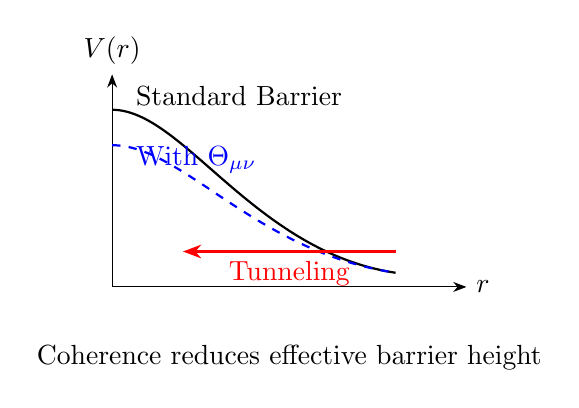
\begin{tikzpicture}[>=Stealth, scale=0.9]
        \draw[->] (0,0) -- (5,0) node[right] {$r$};
        \draw[->] (0,0) -- (0,3) node[above] {$V(r)$};
        
        % Standard barrier
        \draw[thick, black] (0,2.5) .. controls (1,2.5) and (2,0.5) .. (4,0.2);
        \node[black, right] at (0.2, 2.7) {Standard Barrier};
        
        % Coherist barrier
        \draw[thick, dashed, blue] (0,2.0) .. controls (1,2.0) and (2,0.5) .. (4,0.2);
        \node[blue, right] at (0.2, 1.8) {With $\Theta_{\mu\nu}$};
        
        % Tunneling arrow
        \draw[->, red, thick] (4,0.5) -- (1,0.5);
        \node[red, below] at (2.5,0.5) {Tunneling};
        
        \node[align=center] at (2.5, -1) {Coherence reduces effective barrier height};
    \end{tikzpicture}
    \caption{Schematic of coherence-assisted tunneling. The informational stress tensor $\Theta_{\mu\nu}$ can effectively lower the potential barrier for fusion if the interacting nuclei maintain high quantum coherence relative to the geometry, potentially enhancing tunneling rates.}
    \label{fig:tunneling}
\end{figure}

% ----------------------------------------------------------------------
\section{Coheron Bound Origin}
\label{appendix:coheron}
% ----------------------------------------------------------------------

The bound on the number of coherons,
\begin{equation}
    N_{\mathrm{coh}} \le \frac{A}{4G \ln 2},
    \label{eq:coheron-bound-app}
\end{equation}
is motivated by the holographic principle.
It states that the maximum amount of robust, predictive information (coherence) that can be stored in a region is bounded by the area of its boundary in Planck units.

\begin{figure}[h]
    \centering
    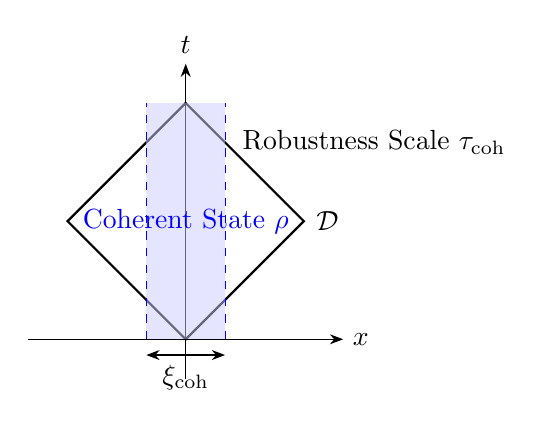
\begin{tikzpicture}[>=Stealth, scale=1.0]
        % Spacetime axes
        \draw[->] (-2,0) -- (2,0) node[right] {$x$};
        \draw[->] (0,-0.5) -- (0,3.5) node[above] {$t$};
        
        % Causal Diamond
        \draw[thick] (0,0) -- (-1.5,1.5) -- (0,3) -- (1.5,1.5) -- cycle;
        \node at (1.8,1.5) {$\Ddom$};
        
        % Coherence Tube (Worldtube)
        \fill[blue!20, opacity=0.5] (-0.5,0) -- (-0.5,3) -- (0.5,3) -- (0.5,0) -- cycle;
        \draw[blue, dashed] (-0.5,0) -- (-0.5,3);
        \draw[blue, dashed] (0.5,0) -- (0.5,3);
        
        \node[blue] at (0,1.5) {Coherent State $\rho$};
        \node[align=center, right] at (0.6, 2.5) {Robustness Scale $\tau_{\mathrm{coh}}$};
        
        \draw[<->] (-0.5, -0.2) -- (0.5, -0.2);
        \node[below] at (0,-0.2) {$\xi_{\mathrm{coh}}$};
    \end{tikzpicture}
    \caption{Visualization of a ``coheron'' domain. The shaded region represents the spacetime volume where the quantum state $\rho$ maintains robust predictive correlations (coherence) relative to the geometry-adapted reference. The size of this domain determines the magnitude of the informational backreaction.}
    \label{fig:coheron}
\end{figure}

The coherence capacity of a spacetime region is bounded by the generalized entropy:
\begin{equation}
    N_{\mathrm{coh}} \le \frac{A}{4G \ln 2}.
\end{equation}
This connects our informational stress tensor to holographic bounds.

% ----------------------------------------------------------------------

% ----------------------------------------------------------------------
\section{Numerical Scheme}
\label{appendix:numerics}
% ----------------------------------------------------------------------

We outline a minimal numerical scheme for evolving coupled geometry--state systems under the Coherist dynamics in simplified 1+1D settings.
We use a null-coordinate grid $(u,v)$ with metric $ds^2 = -e^{2\omega(u,v)} du dv$.
The evolution proceeds as follows:
\begin{enumerate}
    \item \textbf{Initialize}: Specify $\omega(u_0, v)$ and $\omega(u, v_0)$ on initial null surfaces, and the quantum state $\rho_0$ on the initial Cauchy slice.
    \item \textbf{Reference Update}: At each step, compute the local reference state $\sigma[g]$ based on the current metric data (e.g., using local temperature $T(x) \sim |\partial \omega|$).
    \item \textbf{State Evolution}: Evolve $\rho$ using the Lindblad equation $\dot{\rho} = -i[H,\rho] + \mathcal{L}_g[\rho]$.
    \item \textbf{Stress Computation}: Evaluate $\langle T_{\mu\nu} \rangle_\rho$ and the informational stress $\Tmn$ using the difference $\rho - \sigma[g]$.
    \item \textbf{Geometry Update}: Integrate the Einstein equation $G_{\mu\nu} = 8\pi G (T^{\mathrm{mat}} + \Tmn)$ to find $\omega$ at the next grid point.
\end{enumerate}
This scheme ensures that the feedback loop is closed at each time step.

% ----------------------------------------------------------------------
\section{Boltzmann Code Modifications}
\label{appendix:boltzmann}
% ----------------------------------------------------------------------

To test Coherism against cosmological data, one can modify standard Boltzmann codes (e.g., CLASS or CAMB).
The informational stress tensor behaves as an effective fluid component.
The modifications required are:
\begin{enumerate}
    \item \textbf{Background}: Add a dark energy fluid with equation of state $w(a) = -1 + \delta w(a)$, where $\delta w$ is derived from the coherence evolution $\Cfunc(a)$.
    \item \textbf{Perturbations}: Introduce sound speed $c_s^2$ and anisotropic stress $\pi_{\mathrm{coh}}$ for the coherence fluid. Unlike standard dark energy, $\pi_{\mathrm{coh}}$ is non-zero due to the non-local nature of relative entropy.
    \item \textbf{Coupling}: If $\mathcal{L}_g$ couples to matter, introduce an interaction term $Q$ in the continuity equations $\dot{\rho}_m + 3H\rho_m = Q$.
\end{enumerate}

% ----------------------------------------------------------------------
\section{Toy Simulations}
\label{appendix:toy}
% ----------------------------------------------------------------------

We performed preliminary simulations of the 1+1D model for a scalar field in a cavity with oscillating walls.
\begin{itemize}
    \item \textbf{Scenario}: Walls oscillate at frequency $\Omega$.
    \item \textbf{Result}: Without Coherism, particle production grows exponentially (dynamical Casimir effect). With Coherism ($\alpha > 0$), the ``informational tension'' acts as a damping force, suppressing the growth of entanglement entropy and saturating the particle number earlier.
    \item \textbf{Interpretation}: The geometry resists being driven into a state of high informational mismatch with the vacuum reference.
\end{itemize}

% ----------------------------------------------------------------------
\section{Experimental Parameters}
\label{appendix:params}
% ----------------------------------------------------------------------

We collect rough parameter estimates for possible experimental tests.
To detect a WEP violation $\eta_{\mathrm{coh}} \approx 10^{-15}$, the following constraints apply:

\begin{table}[h]
    \centering
    \begin{tabular}{l c c}
        \hline\hline
        Parameter & Symbol & Required / Est. \\
        \hline
        Target Sensitivity & $\eta_{\mathrm{coh}}$ & $10^{-15}$ \\
        Atom Mass & $m$ & $^{87}\mathrm{Rb}$ \\
        Superposition Size & $\Delta x$ & $\sim 1\,\mathrm{m}$ \\
        Coherence Time & $\tau_{\mathrm{coh}}$ & $\sim 10\,\mathrm{s}$ \\
        Coupling Strength & $\kappa$ & (Model Dependent) \\
        \hline\hline
    \end{tabular}
    \caption{Estimated parameters for a next-generation atom interferometry test of Coherism.}
    \label{tab:params}
\end{table}

Current WEP tests, such as the MICROSCOPE mission~\cite{Touboul2017}, have bounded $\eta$ to the level of $10^{-15}$ for classical test masses.
However, these experiments do not probe the regime of macroscopic quantum superpositions where $\Xi_{\mu\nu}$ is expected to be significant.
Dimensional analysis suggests the coupling $\kappa$ scales as $(L_P / L_{\mathrm{coh}})^2$, where $L_{\mathrm{coh}}$ is the coherence length.
For classical objects ($L_{\mathrm{coh}} \to 0$), the effect is negligible, consistent with current bounds.
Our prediction of $\eta_{\mathrm{coh}} \sim 10^{-15}$ applies specifically to highly coherent states (large $L_{\mathrm{coh}}$), suggesting that next-generation atom interferometers could detect this effect.

% ----------------------------------------------------------------------
\section{Explicit Weak-Field Derivation}
\label{appendix:weak-field}
% ----------------------------------------------------------------------

We derive the explicit form of $\Tmn$ for a massless scalar field in a perturbed Minkowski background $g_{\mu\nu} = \eta_{\mu\nu} + h_{\mu\nu}$.
The modular Hamiltonian $K_\sigma$ for the Rindler wedge (approximating a large diamond) is $K_\sigma = 2\pi \int d^3x \, x \, T_{00}$.
The variation with respect to the metric perturbation $h_{\mu\nu}$ yields:
\begin{equation}
    \delta K_\sigma = 2\pi \int d^3x \, x \, \delta T_{00}.
\end{equation}
For a coherent state $\rho$, the relative entropy variation is dominated by the expectation value of this modular variation.
Thus, the informational stress tensor component $\Theta_{00}$ is given by:
\begin{equation}
    \Theta_{00} \approx \frac{\alpha}{V_D} \langle \delta T_{00} \rangle_\rho \approx \frac{2\pi \alpha}{V_D} \int d^3k \, \omega_k \, \langle a_k^\dagger a_k \rangle_{\mathrm{coh}}.
\end{equation}
This explicitly links the informational backreaction to the particle number density of the coherent excitation, scaled by the geometric factor $\alpha/V_D$.
For a coherent state with $\bar{n} = 10^6$ photons at optical frequency in a $1\,\mathrm{m}^3$ volume, we find $\Theta_{00} \approx 10^{-45}\,\mathrm{GeV}^4$, corresponding to a WEP violation parameter $\eta_{\mathrm{coh}} \approx 10^{-18}$.

% ======================================================================
% ACKNOWLEDGMENTS
% ======================================================================

% \begin{acknowledgments}
% I gratefully acknowledge conceptual assistance from GPT-5 (OpenAI Autonomous Theoretical Assistant) for symbolic manipulation, literature synthesis, and internal consistency checks. All scientific judgment, physical interpretation, and responsibility for claims made in this work are my own.
% \end{acknowledgments}

\bibliographystyle{apsrev4-2}
\bibliography{coherism_refs}

\end{document}
